\begin{abstract}
 The abstract goes here... (BITCOIN influence -> Blockchain). Captivate readers attention.
\end{abstract}




%*****************************************
\chapter{Introduction}
%*****************************************

Blockchain (BC) has been considered as one of the most promising disruptive technologies during the last years. Many market-leading companies, experts and global innovators have referred it as the "Next Generation of the Internet" \cite{JenClarck2017}, succeeding the World Wide Web era. Evaluating its potential benefits, different banks and major enterprises, such as UBS, Microsoft or IBM, have already accomplished important investments in such innovative technologies.

The revolution started in 2008, with a whitepaper publication by Satoshi Nakamoto \cite{nakamoto2008bitcoin}, who introduces a new digital payment protocol called Bitcoin. Satoshi Nakamoto is just a name used by an unknown person or group of people to first reference the implementation. Nowadays, Bitcoin's creator still remains a mystery.

In 2009, a deployed software version based on the paper was launched. Bitcoin uses an alternative virtual currency, to make trusted transactions between different peers. This system relies on a kind of distributed database allocated on the Internet, the blockchain. Blockchain uses a peer-to-peer architecture model combined with secure algorithms, such as public key cryptography, which intentionally removes the presence of middle-parties or intermediaries. Thus, in the case of Bitcoin, it eliminates the agent responsible for transactions: central banks.

At the beginning, the blockchain architecture was restricted to only one application: online payments. However, after observing its advantages and possible use cases, an improvement of Bitcoin emerged: Ethereum\footnote{\url{https://www.ethereum.org/}}. By contrast, Ethereum extends the power of decentralized transactions with a Turing-complete contract system. A Turing-complete system can perform any computation, with just writing a few lines of code, in order to create Ethereum scripts: smart contracts. A smart contract can be generated with non-restrictive and user-friendly programming languages, allowing developers to easily learn and benefit from them. Therefore, it brings to the user the opportunity to develop their own applications. Smart contracts are used to implement decentralized apps, which unlike normal web apps, they may not be allocated in a central server. In other words, they use blockchain technology to retrieve and store data instead of a database.


\section{Motivation}

Nowadays, blockchain is becoming a trending topic in the business world. Thousands of articles, research papers and books, such as: How the technology behind bitcoin is changing money, business and the world \cite{tapscott2016blockchain} or Blockchain: Blue print for a new economy \cite{swan2015blockchain}, are catching the public eye. Nevertheless, as it is an emerging technology, a necessity to look towards new horizons exists. Through the use of the above mentioned Ethereum smart contracts new possibilities to approach existing problems are opened up. Hence, blockchain technology can be used in many applications beyond currency.

Many scenarios are currently investigated from a blockchain perspective, e.g: candidate's voting or asset tracking \cite{abeyratne2016blockchain}. In the former, voters send signed and encrypted ballots to the blockchain contract, who immediately verifies them. Simultaneously, it also preserves confidentiality, since the ballot can only be emitted from its owner. In the latter, each physical asset could be encoded in the blockchain enabling a fast and transparent tracking. For example, Everledger\footnote{\url{https://www.everledger.ioafa}}, a startup company from London, tracks diamonds storing each diamond's digital identity on the BC. Thus, diamond theft could be effectively prevented.

After investigating the implementation of blockchain in real scenarios, one top-level application is clear: it can be used as a software connector. Blockchain contributes to face security, storage's problem, communication and coordination between users. In this paper, we will focus on enterprises or organizations, suffering from such problem, referenced from now on as supply chain challenges.

\section{Problem Statement and Contribution}

Supply chain management is the process of linking organizations through information flows, in order to achieve a competitive strength or advantage, which will maximise customer value. Supply chain activities go from the design or development of a product, up to its return on investment (ROI). Thus, a good coordination during these activities is extremely needed.

Nowadays in the Big Data era, enterprises must handle a huge amount of information. This leads companies to suffer from considerable issues, such as scalability, data's security or communication. One could think that currently most of these companies rely on third parties, which help them on the mentioned problems. But what if this process could be efficiently accelerated in a secure and decentralized manner? Here, is where Blockchain can play a crucial role.

During the paper, the focus will be on IT companies facing this dilemma. The scenario will include in one side different customers, and in the other organizations acting as providers. For example, eBay, one of the biggest multinational e-commerce corporations, acts as an intermediate for the product's purchase-sale. Thus, eBay is responsible for managing all this data. However, can a user/company always safely trust third-parties? Why not using BC as the main responsible for handling such complex tasks? This will result in a direct customer-provider relation, avoiding the presence of any intermediaries.

For this scenario, a current application example that consists of the embedding of virtual networks (network virtualization) between different Infrastructure Providers (InPs), will be further investigated \cite{dietrich2015multi}. This process can also be called network slicing. In this example, Service Providers (SPs) want to embed virtual nodes among different InPs in order to provide wide-area network services. Nevertheless, Infrastructure Providers are not willing to publicly disclose its internal network topology, along with its resources availability and costs. In such cases, brokers, usually known as VN Providers (VNP) try to perform the embedding under the mentioned limited information disclosure (LID) problem. As a result, it can be clearly observed that blockchain can solve this interaction, providing: secure sensitive data storage, customer-provider negotiation without third-parties (without VNP) and finally maintaining a coordinated process. The negotiation between the involved parties will be based on a time-limited auction system, where each virtual network request will be stored as a contract on the blockchain network.

Therefore, a good question for the theses could be: How blockchain takes advantage of distributed workflows providing an agile and secure environment? Exemplifying workflows, with the network slicing example. At the end, a decentralized application approaching the mentioned problem will be deployed. In addition, the app will include a user-friendly front-end in order to guide users through the process. 

\section{Outline}

This thesis is structured as follows. In Chapter \ref{ch:background}, relevant background on blockchain, network virtualization and auction mechanisms is given. Afterwards, an overview and analysis of existing research about blockchain in supply chain management and multi-provider virtual network embedding is presented in Chapter \ref{ch:relatedwork}. Based on these investigation, in Chapter \ref{ch:design} an application system design to solve the virtual network embedding problem using blockchain is exposed. Then, the implementation of the proposed design is discussed in Chapter \ref{ch:implementation}. The created application along with its technologies are tested from different perspectives in Chapter \ref{ch:evaluation}. Last but not least, in Chapter \ref{ch:closure}, the conclusions of this thesis are exposed as well as possible improvements for future work.


%*****************************************
\chapter{Background}
\label{ch:background}
%*****************************************

In this section, an overview of the blockchain technology evolution will be provided. It starts with the 1st blockchain generation related to cryptocurrencies, with Bitcoin as a leading representative. Then, the second or smart contracts generation will be investigated, where Ethereum extends the idea of money transfers, to any other application that can be writable as a piece of code.

Afterwards, the network virtualization concept will be introduced, in which resource negotiation between customer and providers is crucial. Due to this importance, a well-known public negotiation mechanism will also be presented: the auctions.

\section{Blockchain: A decentralized and distributed trustless ledger}

A blockchain is a decentralized distributed ledger, which stores the entire history of transactions on the network. In other words, it is a simple database distributed among a network of computers, where each computer has an identical copy of this database. This contrasts with traditional (e.g. SQL) databases that are controlled by a single entity. Thus, in a blockchain, there is no central server or agent in the middle of the communication. For example, imagine a user willing to transfer money to another one \ref{fig:CentralizedvsDecentralized}. In a centralized system, the transaction will go first to the bank, who will update its internal database and subsequently perform the operation. In contrast, by a decentralized system, each user is able to directly transfer the money, since it possesses an updated copy of the database. Another example to replace a centralize design could be in the healthcare environment. There, patient records are stored in multiple databases, which always leads to a costly exchange of information between them. In this scenario, the blockchain could improve the process, preserving patients confidentiality in a secure and decentralized manner.

\begin{figure}[bth]
	\centering
	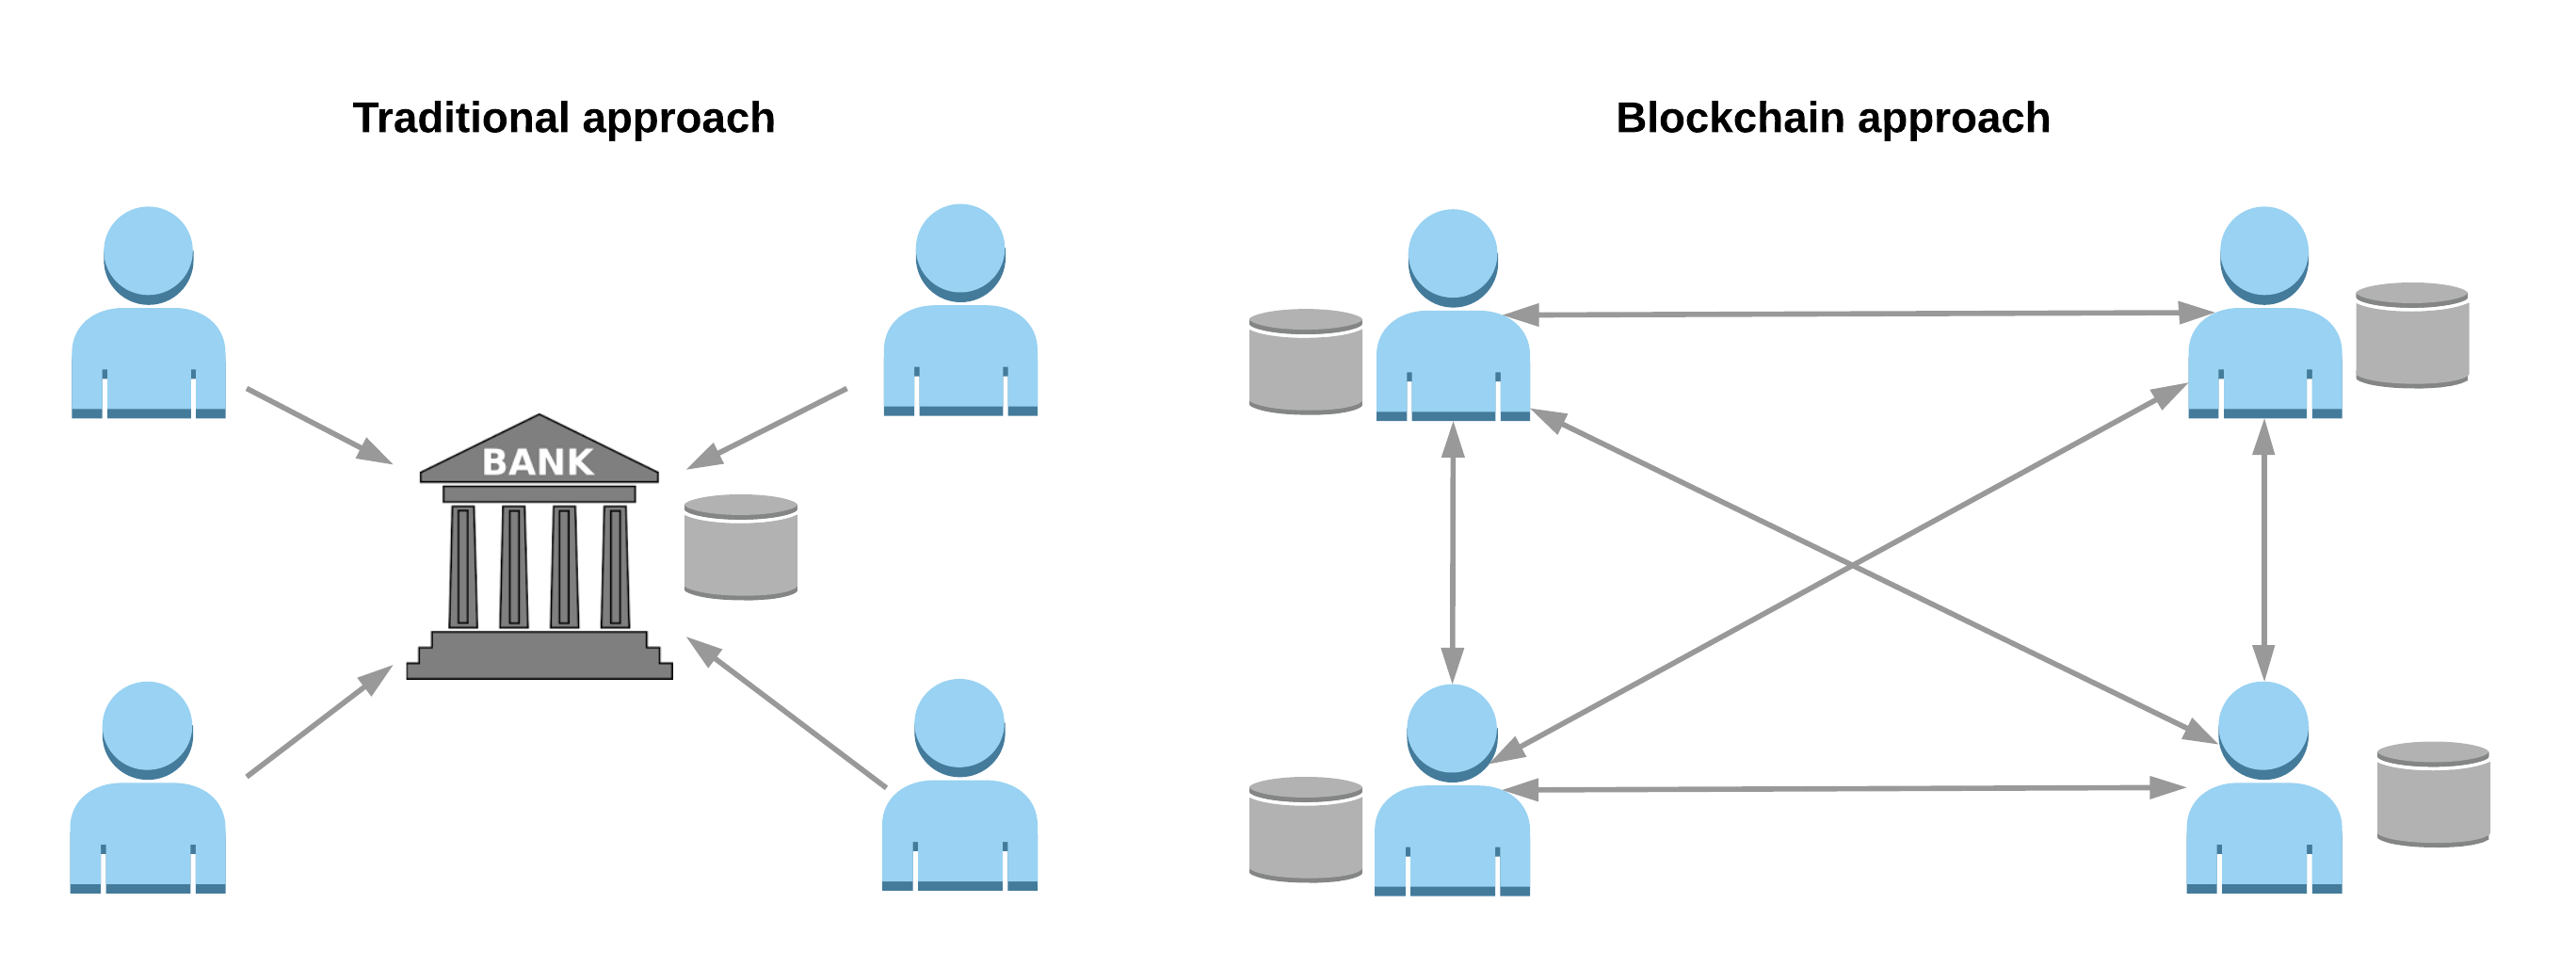
\includegraphics[width=0.8\linewidth]{gfx/cenVsDec}    
  	\caption{Traditional database vs blockchain approach}
  	\label{fig:CentralizedvsDecentralized}
\end{figure}

At the beginning, the terms Bitcoin and blockchain were sometimes interchanged, as these words were used to refer: (i) the technology, (ii) the protocol for making transactions and (iii) the cryptocurrency (money). Therefore, before continuing, one statement needs to be clear: Bitcoin is a cryptocurrency that uses the blockchain technology. Hence, Bitcoin is just one of the multiple applications that use blockchain. 

However, when a new technology appears, the first user's goal is normally to exploit its economic potential. For this reason, money transaction through cryptocurrencies was its first application. In the next subsection, we will understand what cryptocurrencies are, followed by an explanation of the Bitcoin's design architecture.

\subsection{Blockchain 1.0: Cryptocurrencies}

At of the end of January 2018, Coinmarketcap\footnote{https://coinmarketcap.com/}, a cryptocurrency market tracker, lists more than 1,400 cryptocurrencies with an aggregate value approaching USD 700bn. But what are cryptocurrencies? Cryptocurrencies are a variety of digital currencies pretending to work as a medium of exchange, such as Euro or USD does. As the name suggests, apart from being a virtual currency, they use cryptography to secure and verify its transactions. The main difference with traditional currencies is that they do not have any physical equivalent in the real world. Nevertheless, they can be used to pay goods and service, with the advantage of not being constrained with geographical or political borders. For example, GMO Internet\footnote{https://www.gmo.jp/en/}, a Japanese company, will start paying parts of employees salaries in cryptocurrencies (Bitcoin).

In this paper, we will set aside whether they can become true currencies or not, and also its political, social or economic impact. The only focus will be the technology behind it, as blockchain can be extended to much more than digital currencies. Thus, we will start from the genesis of the technology, with Bitcoin as its revolutionary innovator.


\subsubsection{Bitcoin}

Bitcoin took the world by surprise in 2008, after Satoshi Nakotomo's white paper publication \cite{nakamoto2008bitcoin} and later its software release. Bitcoin (BTC) is a cryptocurrency used for making secure transactions across a peer-to-peer (P2P) network. In addition, Bitcoin uses its own protocol that operates in an overlay network, the blockchain. An overlay network is a computer network build in the top of another network, in this case above Internet application's layer, which is controlled by its users (no central authority).

From another point of view, the Bitcoin ledger can be interpreted as a state transition system, where there is an initial state, which after a transition function (money transfer), results in a new state. Imagine an scenario where user A wants to send 10 BTC to user B. The first state is A and B current balance and the transition function will take 10 BTC from A and insert it to B's account, generating a new state. But what happens if A sends exactly the same payment to two different addresses (B and C) at the same time? This scenario is the so-called \textit{double spending attack} and consequently, a transaction always needs to be verified by miners before being confirmed. 

\paragraph{Mining and Transactions}

Miners are specific blockchain users, responsible for monitoring and verifying all the transactions between users. And how all these miners cooperate efficiently? The answer to this question is one of the most remarkable Satoshi innovation key factors, which consists of the communication between nodes through a simple decentralized consensus protocol. This consensus protocol consists of multiple algorithms (e.g. Proof of Work), used by the miners in the Bitcoin network.

Therefore, Bitcoin needs to combine the state transition system with a consensus protocol, in order to synchronize the order of all transactions among the users. There, new transactions are stored in the last block of the blockchain, and a new block is mined every ten minutes. Over time, this creates an ever-growing chain of blocks, which are constantly updated. Thus the name: blockchain. Additionally, a complete history of the transactions is kept, so everyone can verify the last money movements. For instance, a blockchain can be compared to an endless domino game, where all the pieces are placed in vertical one after the other. Each of these pieces references a block, and if one block is removed (e.g. transaction error), all the subsequent ones will be affected. Hence, as miner's task is not simple and requires computational power, if they are the first block solvers, they are also economically rewarded. Additionally, if any transaction has a positive balance at the end, it is also destinated to the miner.

Figure \ref{fig:Blockchain mining} shows how transactions are bundle into blocks, where each block contains a:

\begin{figure}[t]
  	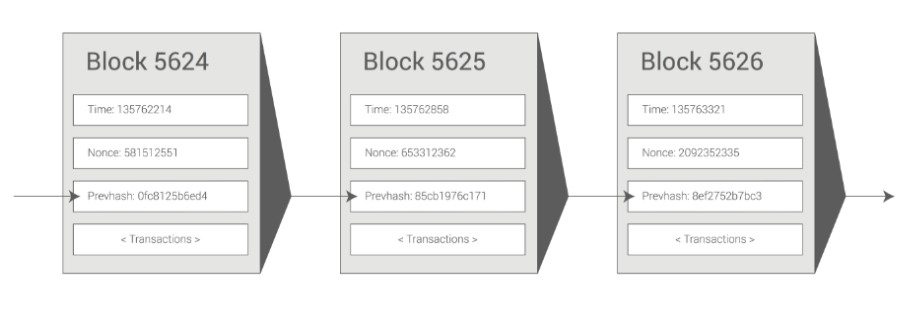
\includegraphics[width=1\linewidth]{gfx/mining}    
  	\caption{Blockchain Mining}
  	\label{fig:Blockchain mining}
\end{figure}

\begin{itemize}
	
	\item Timestamp, to identify when the event occurs.
	\item Nonce used to avoid malicious nodes from flooding the blockchain.
	\item Hash of its previous block, to keep track of already added blocks. 
	\item A list of all the transactions that have been created since the previous block. To save storage, this transaction list is typically stored in a a Merkle tree \citep{merkle1987digital}.
\end{itemize}

Furthermore, in Bitcoin, each block and transaction is restricted to a size of 1MB and 250-300bytes respectively, and for a block being valid it needs to satisfy the following requirements:

\begin{itemize}
	
	\item Previous block referenced exists.
	\item Block's timestamp is greater than previous block one.
	\item Proof-of-work in this block is valid.
	\item If any transaction from the transaction lists returns an error, exit.
	\item If all previous steps confirmed, store state at the end of the block and return true.
\end{itemize}  

In the third step of the block validation process, appears the term \textit{Proof-of-work}. Bitcoin uses the Hashcash proof of work algorithm to prove that a block miner spent some computational time creating a block. More precisely, Bitcoin protocol demands that miners find an input, which is a valid $block \, header$ formed by a random value ($c$) and nonce ($x$), whose cryptographic hash (e.g $SHA256$) is less than a determined value. This value is obtained from $d$, the blockchain difficulty. Then, the only way to create a valid block is simply trial and error until a valid Proof-of-Work is generated. Proof-of-work is also used in other contexts, such as for limiting email spam or denial-of-service attacks (DoS).

$$ F_d( \, block \, header \,) = F_d( \,c,x \,) = SHA256( \, SHA256( \, c|x \,) \,)\, < \frac{2^{224}}{d}$$

\paragraph{Key management}

In Bitcoin, each user is identified by a single public address. However, how is this Bitcoin address generated? This process involves the following steps:

\begin{enumerate}
	
	\item A random 256-bit private key is created. Since this key will be used to sign the transactions, it must be kept secret.
	\item A 512-bit public key is generated from the private key, using the Elliptic Curve Digital Signature Algorithm (ECDSA\footnote{\url{https://www.maximintegrated.com/en/app-notes/index.mvp/id/5767}}). This key is used for verifying private key signatures.
	\item This public key is hashed to 160 bits using SHA-256/RIPEMD. Apart from size constraints, the reason for hashing the public key is that if there is a vulnerability in elliptic curves, user's money can still be safe, since only the hash is known.
	\item Finally, the public key is encoded in ASCII using Base58Check. This output is the resulting Bitcoin address.
	
\end{enumerate}

\begin{figure}[bth]
  \centering
  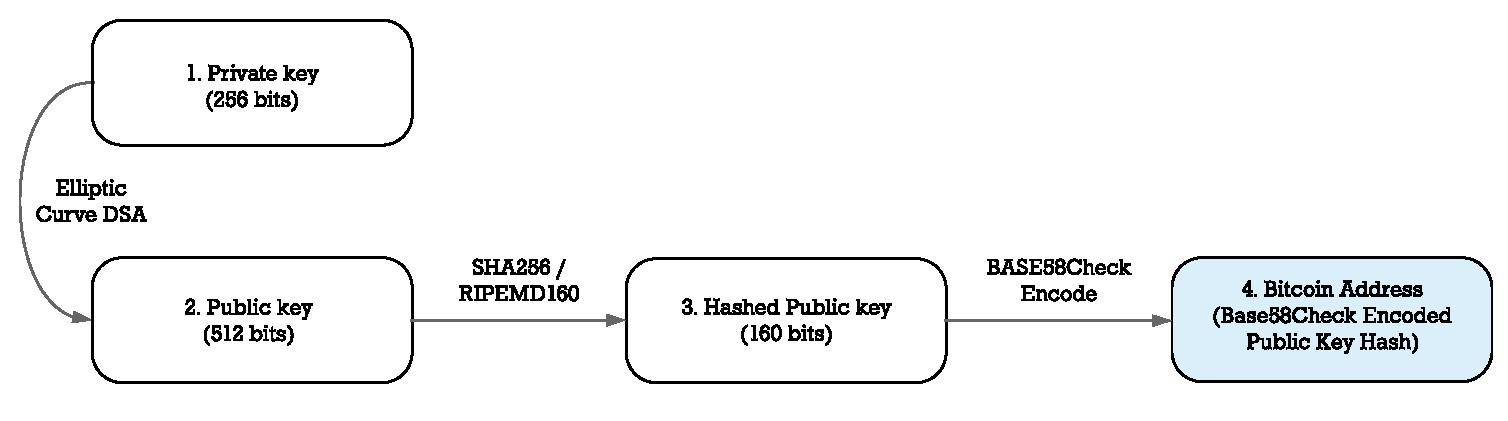
\includegraphics[width=0.9\linewidth]{gfx/bitkeys}    
  \caption{Bitcoin keys and addresses relation \citep{BitcoinKey2018}}
  \label{fig:EthereumAccounts}
\end{figure}

After that, users are able to send transactions using Bitcoin. For example, imagine the last example where user A wants to send 10 BTC to user B. Firstly, the user creates a transaction willing to transfer 10 BTC to user address B. Secondly, he signs the transaction with his private key, attaching also his public key, and sends it to the blockchain. There, miners will verify the signature using A's public key and also that its hash matches user A address. If both, the signature and the hash, are correct, the transaction is accepted and added to the next block. Transactions examples can be found in Block Explorer\footnote{\url{https://blockexplorer.com/}}.

\subsection{Blockchain 2.0: Smart contracts}

The Blockchain 1.0 had numerous limitations since essentially it only approaches the decentralization of money and payments. However, the architecture implemented by Bitcoin is extensible beyond financial uses cases.

\subsubsection{Ethereum}

In 2013 Vitalik Buterin, a Russian-Canadian programmer released the Ethereum white paper \cite{buterin2014next}, where he describes an alternative platform running in a blockchain that allows building any kind of decentralized application. In 2014, Ethereum started as a crowdfunding project, which collects small amounts of money from a large number of users. Currently, Ethereum is a running project and the second most valuable cryptocurrency.

Furthermore, it is built on a Turing-complete contract system. As previously explained, a Turing-complete system allows the developer to perform any computation, which runs on the so-called \textbf{smart contracts}. These smarts contracts are executed by the Ethereum nodes, each using its Ethereum Virtual Machine (EVM), or in other words, a blockchain with a built-in programming language.

In the end, smart contracts are basically Ethereum scripts that whenever they are called, the function programmed inside of it is executed. A smart contract can also be seen as the logic inside a vending machine. For instance, a buyer wants a Coke bottle that costs 2 \euro.. Once this buyer inserts 2 \euro and presses the button, a small program (contract) runs inside the vending machine and supplies the user with its Coke. This function, in the smart contract context can be seen as:
\newline
\begin{lstlisting}
 if (button_pressed == 'Coke' && rcv_money == '2')
 	return coke
\end{lstlisting}

Therefore, smart contracts allow anyone to write their own functions, in just a few lines of code. Despite Bitcoin and Ethereum have similar features, such as decentralization or transaction-based, Ethereum makes use of smart contracts, which potentially opens up real-world use cases. Bitcoin and Ethereum can be comparable to a calculator (one application) and a smartphone (multiple applications) respectively. In addition to the already mentioned, there are several differences that need to be highlighted:

\begin{itemize}
	
	\item Ethereum's block time is shorter, specifically around 14s. Remember that Bitcoins mining time was around 10 minutes. Hence, as a consequence, Ethereum needs to handle extremely large amounts of transactions in seconds, which means that the network can easily get stuck with different subchains. To solve this scalability issues, Casper, a new consensus strategy has been recently deployed \cite{proofOfStake}.

	\item Bitcoin's blocks and transaction sizes are indicated in bytes, however, in Ethereum, it depends on the contract complexity. This complexity is expressed in terms of gas, which is the amount of ether \footnote{ether or ETH is the digital currency used by Ethereum}, used for executing contracts in the Ethereum blockchain. 
	\item Ethereum moves from the Proof-of-Work to the Proof-of-Stake (PoS) concept. In contrast to PoW, where the miners that first solve a mathematical problem are rewarded, in PoS, the block's creator is selected in a deterministic way (wealth depending or stake). Also, a miner does not receive a block reward, but instead he earns all gas used for executing the smart contract.
	\item Ethereum transactions compared to the mentioned Bitcoin fields consists of (i) the transaction value in Ether, (ii) recipient address, (iii) data arguments and (iv) execution cost.
	\item Ethereum is account-based and not transaction-based.
\end{itemize}

In the last point, we observe that Ethereum introduces a new concept called accounts. These accounts are unique 20-byte addresses in the blockchain, each of them having a balance controlled by ethers (ETHs). In Ethereum, there are two types of accounts (Figure \ref{fig:EthereumAccounts}):

\begin{itemize}
	
	\item \textbf{Externally Owned Accounts (EOAs):} These accounts normally identify a user, being controlled by their own public and private keys. Only EOA can send transactions to other accounts. A transaction in Ethereum can either send Ethers or call/trigger a contract account  
	\item \textbf{Contract accounts:} These are the accounts, where the code (smart contract) is stored. Thus, once triggered (function call from another contract), its defined code is executed.
\end{itemize}

\begin{figure}[bth]
  \centering
  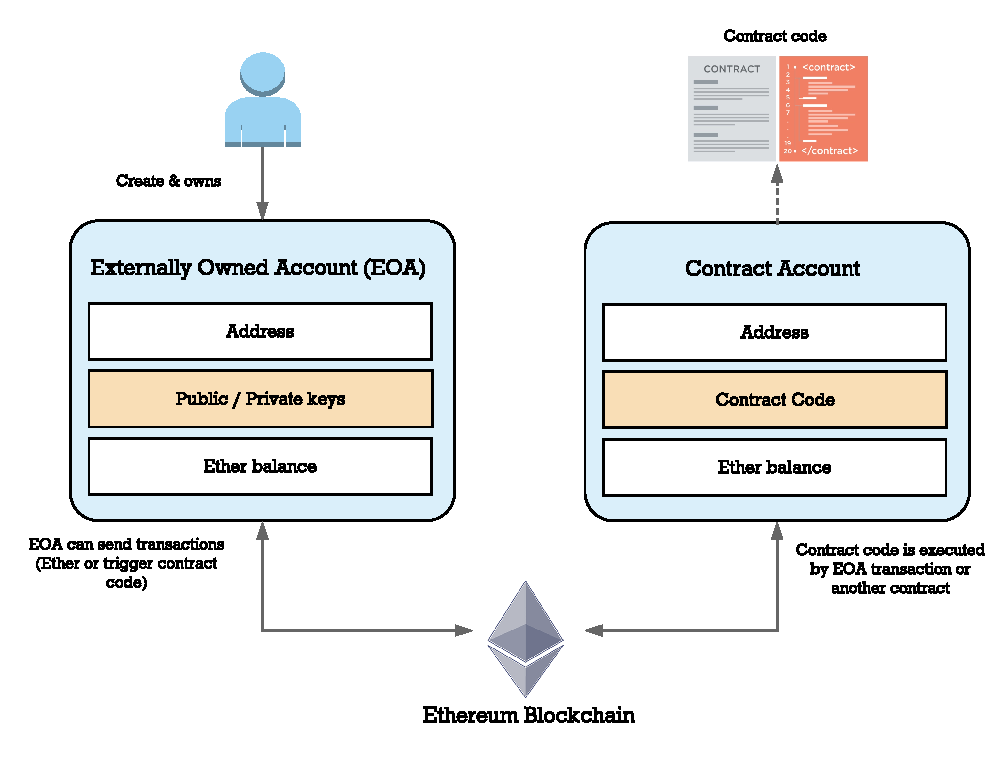
\includegraphics[width=0.6\linewidth]{gfx/ethereumAccounts}    
  \caption{Ethereum accounts: Externally owned accounts and contract 			accounts}
  \label{fig:EthereumAccounts}
\end{figure}

However, what happens if this contract code results in an infinite loop? The node will get stuck the whole time executing this contract. Thus, Ethereum uses the above-mentioned term: gas. For example, suppose an EOA calling a contract account for money transfer. Apart from the ether transferred, it will also spend an additional amount of ether (gas). Thus, the ether used for a transaction, or transaction fee is:

$$Transaction\ fee = gas price \times gas limit + value - unused gas$$

Firstly, the $gas limit$ is the maximum amount of gas that a sender is willing to spend on a transaction. By default 21000 is the minimum gas limit for all
transactions. Fortunately, all $unused gas$ during a transaction ($gas limit - real gas used$), is refunded to the sender. Nevertheless, if a transaction gives an error, e.g: a fake transaction, this provided ether (gas limit) will never be refunded. Secondly, the $gas price$ is its relation with real Ether, e.g: 40 Gwei (4e-8 ether). Thirdly, the $value$ is the amount of ether transferred to the other EOA.

In conclusion, a smart contact is just an account containing code, which lives on the blockchain and allows developers to create their own decentralized applications. 

\subsubsection{Decentralized applications}

In the Ethereum white paper \cite{buterin2014next} dapps are split into three types. The first group includes financial applications, where users exchange ether in an efficient and distributed manner. The second group is formed by semi-financial applications, in which money is involved but it is mixed with data from the real world, for example with weather feed. And finally, in the third category, there are non-financial applications. For instance, an online voting platform providing a better transparency into elections, without compromising voter confidentiality.

Despite the blockchain is a secure technology, its created applications are constantly compromised to multiple attacks. This is because the majority of smart contracts are insecure, due to its code being prone to bugs.
For example, in June 2016, the DAO\footnote{https://ethereum.org/dao}, a distributed autonomous organization instantiated on the Ethereum blockchain, was hacked. The attack, which was a smart contract bug, had resulted in over 50 million dollars of cryptocurrency theft. Thus, smart contracts need to be protected against malicious attacks before being uploaded on the blockchain.

In the following section, an example application or process currently performed by IT companies will be introduced.


\section{Network Virtualization} \label{networkvirtualization}

In the last few years, network virtualization has started to grow in popularity since it enables simulating hardware networks, in software. These software networks are called virtual networks, and in contrast to physical networks, they provide flexibility, manageability and a low cost. 

Network virtualization handles two main concepts: node virtualization and link virtualization. The former implies sharing the node's physical resources located in the substrate network (e.g: CPU, storage, memory) to multiple virtual nodes in the virtual networks, such as physical node A in Figure \ref{fig:networkvir}.a. The latter enables the transport of multiple virtual links in a single and shared physical link (Figure \ref{fig:networkvir}.b).

\begin{figure}[bth]
  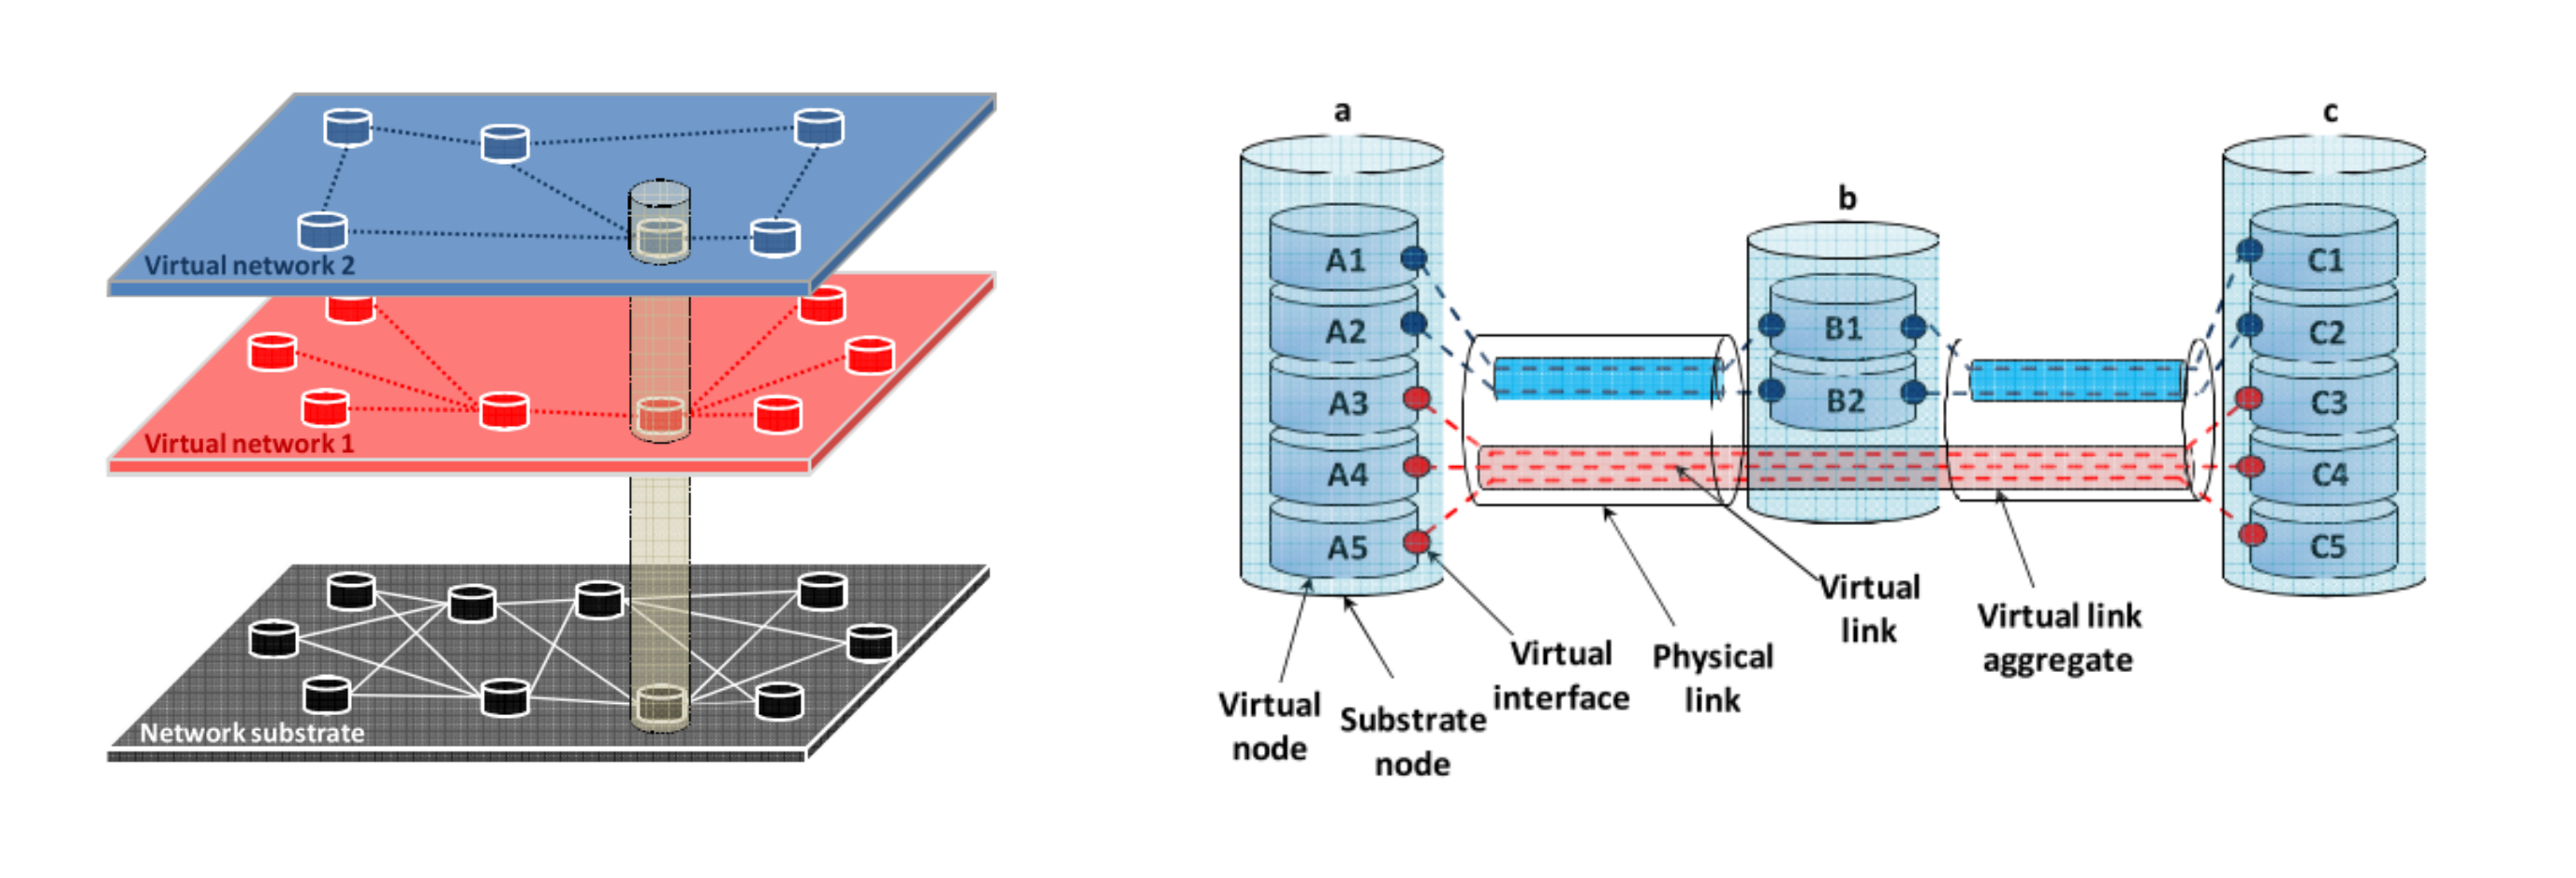
\includegraphics[width=1\linewidth]{gfx/networkvir}    
  \caption{Network virtualization model and its basic elements \citep{carapinha2009network}}
  \label{fig:networkvir}
\end{figure}

In a real scenario, there are two main actors (and one optional) participating in the network virtualization process.

\begin{itemize}
	
	\item \textbf{Infrastructure providers (InPs):} Infrastructure providers (e.g: Deutsche Telekom or Telefonica) deploy and manage the physical nodes, sharing efficiently its resources to the virtual network. For InPs, this results in a significant decrease in operational and technology investment costs \citep{dietrich2015multi}.
	\item \textbf{Service Providers (SPs):} Service providers lease virtual resources from infrastructure providers to create its customized virtual network. All this without the need to purchase physical network equipment.
		\item \textbf{Virtual network providers (VNPs):} Are the brokers, which can optionally serve as intermediaries between the infrastructure and service providers.
\end{itemize}

The network slicing process with the presence of a broker typically starts with the VNP obtaining the necessary information from the InPs. This data will be used to divide the virtual network into groups of nodes (subgraphs). Thus, once the SP sends a VN request, this is immediately optimized (in terms of cost) by the VNP. Afterwards, the modified request is transmitted to the multiple InPs, who are in charge of allocating the virtual nodes from the request in their physical resources. 

The presented process is coordinated by an actor, the VNP, who stores all the information to successfully allocate the incoming resources. However, there are other approaches which do not rely on a central entity. Conversely, they use a consensus mechanism between the SPs and InPs to perform the virtual resources trading. Thus, in the following, we will briefly investigate an open negotiation technique: the auctions.

\subsection{Auction Mechanisms} 

An auction is a public negotiation method involving buyers and sellers that enables resource trading between P2P users. While buyer's goal is to find the desired service at the lowest price, providers or seller's goal is to catch the attention of buyers who are able to pay the highest price for its offered services. Thus, an auction must provide fairness in terms of technical and economic efficiency, for both the buyer and the seller.

Firstly, auctions can be divided into (i) \textit{one-sided auctions} where only the buyers submit their bids (e.g: a painting auctioned in an art auction), or (ii) \textit{two-sided auctions} in which buyers and sellers submit their bids. Normally, when any of the two sides (buyer or seller) cannot perform a good estimation of the service, a one-side auction is preferred. This is the case in network virtualization, where the SPs are not aware of the InPs physical nodes availability or complexity. Secondly, the auctions are (i) \textit{open cry} auctions, where the bids are broadcasted to all users (traditional type), or (ii) \textit{sealed-bid} auctions in which bidders first commit bid values in secret that are later revealed (e.g: physical envelopes). In our scenario, the InPs should bid in a confidential manner, because they do not want to disclose internal data. 

Therefore, according to the above-mentioned auction types, a \textit{sealed one-side auction} is the most suitable in network virtualization.

\subsubsection{Vickrey Auction Model} \label{vickrey}

Many types of auction models exist, such as the English or Dutch auctions \cite{coppinger1980incentives}, however, as we need a sealed-bid our focus will be on a particular one: the Vickrey auction model \cite{vickrey1961counterspeculation}. The Vickrey auction model is considered a fair-price system since it provides a reasonable price to the buyer by motivating bidders to bid truthfully. One of the Vickrey auction model important aspects is that corresponds to a \textit{second-price} auction. In a second-price auction the bidder will offer a price for the service, and among all the bids, the highest one will win the auction. Nevertheless, unlikely standard auctions, the service will be rendered at the second highest bid. For example, if the winning bidder bids 15 \euro and the second highest bid is 10 \euro, the winner pays only 10 \euro. From the bidder point of view means that he can safely bid the true value, knowing that if he wins, he will pay less than his bid. 

However, the second-price concept needs to be thoroughly investigated as long as a bidder can submit multiple bids. Imagine an scenario, where a single bidder A submits two bids: \{1 \euro,9 \euro\} for a service with a real cost 5 \euro. In this case, this buyer will end up paying 1 for the service. Therefore, the second-price auction model needs always to be compared between bidders and not between bids. Suppose the last example, with a second bidder B submitting \{5 \euro, 6 \euro\}. At the end user A, will win the bid but paying 6 \euro, risking that if he would have been the only user bidding, he would have payed 9 \euro.

Ultimately, after judging the preceding analysis of each auction type and model, the \textbf{\textit{second-price sealed-bid}} or simply the \textbf{\textit{Vickrey auction}} fulfills the network virtualization requirements, providing confidentiality and the highest aggregate profit among sellers and buyers.

\section{Summary}

The blockchain is a transparent, secure and robust system where users are in charge of their own accounts and transactions. Beyond money transfer, which starts with Bitcoin, the blockchain technology can be used as a software connector in multiple scenarios. Due to smart contracts, any kind of application could be implemented, enabling developers using the BC concept in their own environment. In the next chapters, the already presented network virtualization scenario will be further investigated.

%*****************************************
\chapter{Related Work}
\label{ch:relatedwork}
%*****************************************

In the following, we explore some of the noted challenges that organizations encounter during their supply chain management (SCM) process, and how they currently approach these issues. Then, we will introduce a recent application in manufacturing, to demonstrate how blockchain could improve SCM efficiency. Henceforth, we focus on a particular supply chain management example: virtual network embedding across multiple InPs. A comprehensive overview of related work on already implemented centralized and decentralized frameworks will be presented. Finally, we will first enumerate the main blockchain benefits observed from the SCM manufacturing application, and secondly, we will analyze the pros and cons of the existing VNE related work, in order to observe the main problems and limitations that need to be addressed in our thesis.

\section{Blockchain in Supply Chain Management}

In the last years, managing the information during the lifecycle of a product represents a major challenge for all companies \citep{karkkainen2003product}, \citep{tuttle2002you}. This product information is constantly changing and in addition, it has to be accessible by different entities. As a consequence, this problem results in high costs for companies. 

Typically, companies approach the problem: (i) storing and maintaining its data into their company-specific infrastructures, which is then communicated to the other supply chain partners, or (ii) sharing this data in a centralized database. In the former, each enterprise creates its own copy of the product data, using their own protocols and procedures.  As a consequence, lots of information asymmetries are found, which ends up destroying the benefits of knowledge or data sharing. In \citep{lee1992managing} and \citep{fiala2005information} inadequate definition of customer services, poor coordination or organizational barriers are named to be some of the pitfalls that these users suffer from. On the other hand, the latter is a great solution as long as the companies trust the party who is maintaining the database. However, what if they are not willing to place this intermediary on their operations? Here, we foresee that blockchain could improve the process supplying data distribution and storage among these companies.

Apart from the supply chain, \citep{heikkila2002supply} states another relationship between suppliers and customers, the Demand Chain Management (DCM), where we predict that blockchain could also play a significant role. In a DCM, the aim is to provide a customer service at the least cost. Hence, the suppliers need a real-time visibility of customer situations and needs. The main difference is that in SCM, the stakeholders wait to receive the order for proceeding with a product (push), whereas in DCM the suppliers observe and immediately operate in user's petition (pull) \citep{wust2017you}. Currently, companies such as Everledger or Skuchain\footnote{\url{http://www.skuchain.com/}}, offer blockchain services to manage and improve the supply chain performance.
 
In the following section, a blockchain application for a manufacturing supply chain system will be presented.

\subsection{Blockchain Ready Manufacturing Supply Chain} \label{manufacturing}

In this part, a blockchain example \citep{abeyratne2016blockchain}, which stores and distributes specific product information during its lifecycle, will be discussed. This task also named product lifecycle management (PLM \citep{stark2015product}), involves different stages in which multiple parties modify the product data. Figure \ref{fig:supplyChain}.a shows the typical stages on this cycle. In this scenario, each actor interacts with a user interface, which is connected to the product's data from the blockchain. Each product is created in form of rules (smart contract) so that only specific users can access or modify this information. To access or insert data into the contract, parties must authenticate themselves signing the request with their private keys. During the lifecycle management, a product is owned by an entity (e.g. distributors). Moreover, when a product goes to another actor (e.g. from distributors to a consumer), both parties will sign a contract that updates product's ownership. Thus, the system guarantees that only the granted user can modify the contract in each phase.

In \citep{abeyratne2016blockchain}, an example is also presented to better explain the mentioned approach. The application consists of the product lifecycle of a cardboard box, starting from the trees cut down until the box is recycled, in which the involved parties are previously registered to the system. In Figure \ref{fig:supplyChain}.b an overview of the implemented design is presented. In this business process, different actors are entailed. For instance, the box manufacturer first receives the physical object and then signs a contract to gain the product's access. Afterwards, he will be allowed to alter the product data through the software application (e.g. box quality). In the end, he will transfer the package (signed) to the next actor, in particular, the product filler.

\begin{figure}
	\centering
	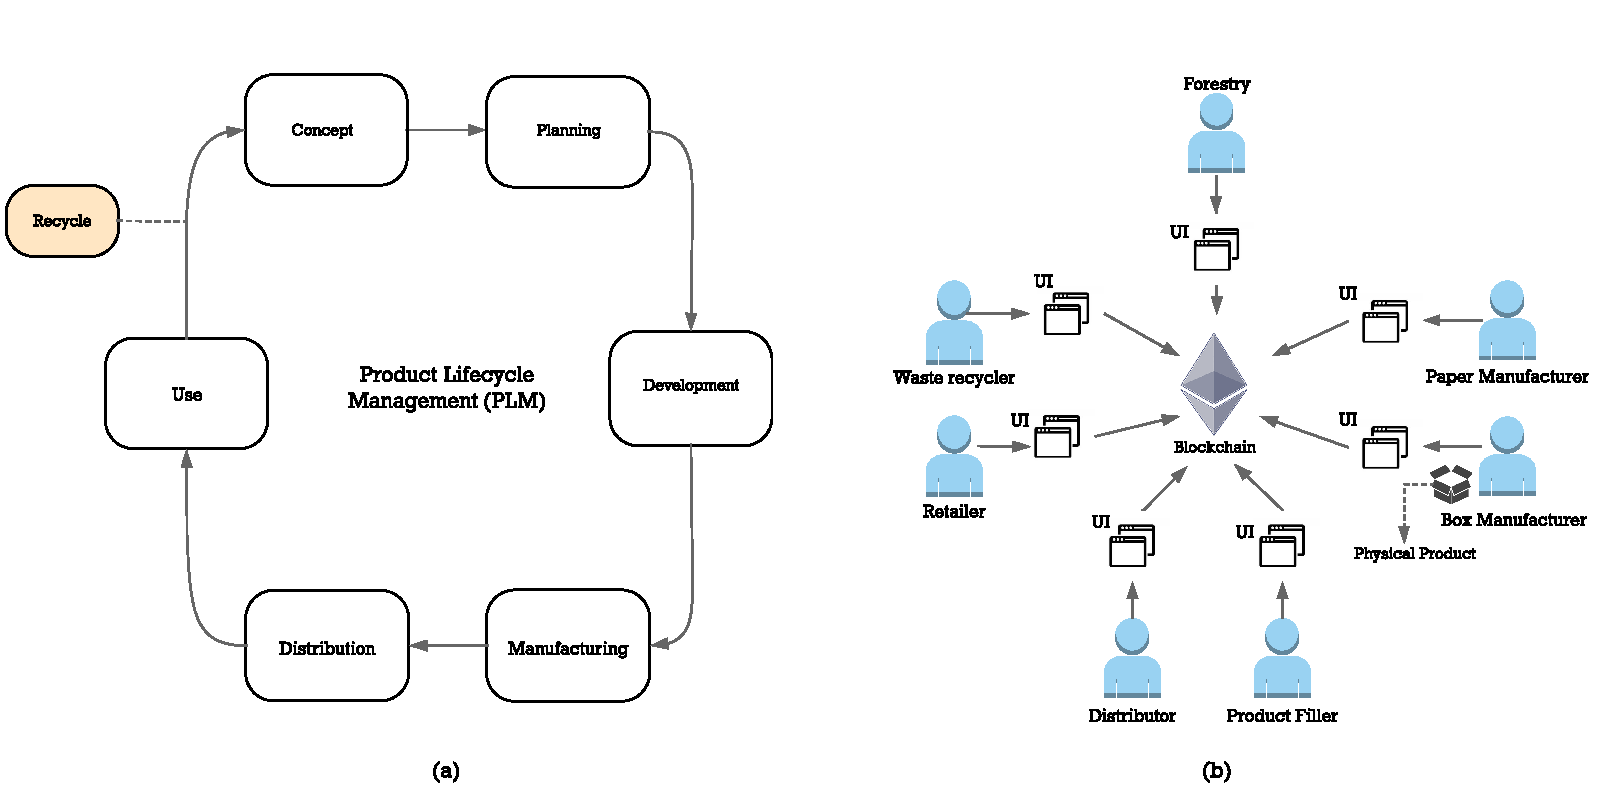
\includegraphics[width=0.9\linewidth]{gfx/supplyChain}    
  \caption{ PLM stages and cardbox blockchain application example \citep{stark2015product}}
  \label{fig:supplyChain}
\end{figure}

\section{Network virtualization}

In the last years, many investigations in network virtualization have been conducted by different authors \citep{houidi2011virtual}, \citep{zhu2008cabernet}, \citep{chowdhury2009virtual}. Among these, it is important to highlight topics such as the trade-offs between single \citep{chowdhury2009virtual}, \citep{houidi2008distributed} and multi-provider VNE \citep{dietrich2017multi}, or the different techniques and algorithms used for achieving VN efficiency. Typically, they decompose the VNE into two tasks: VN partitioning and VN segment mapping \citep{fischer2013virtual}. 

Each of these studies proposes new interesting features compared to the prior research. Nevertheless, in this paper, we will not contrast the different architectures (e.g. between a single or multiple InPs) or discuss the various VN partitioning and mapping algorithms. The main goal of this work will be to explore an existing network virtualization scenario, in particular, multi-provider VNE applications suffering from the limited information disclosure problem or LID \citep{dietrich2017multi}, \citep{zaheer2010multi}, \citep{esposito2013general}, \citep{chowdhury2010polyvine}.

\subsection{Multi-Provider Virtual Network Embedding with Limited Information Disclosure}

To deploy wide-area networks, service providers are willing to embed virtual resources across heteregeneous domains belonging to different infrastructure providers (Figure \ref{fig:multi}). As a result, the system avoids being restricted to just a single provider topology, providing at the same time better efficiency. This process, also named inter-domain VNE\footnote{inter-domain is between multiple InPs and intra-domain is inside a single InP.}, is descomposed in three main tasks \citep{chowdhury2010polyvine}:

\begin{itemize}
	\item \textbf{VN request partitioning}: Divide the virtual network into groups of virtual nodes (subgraphs), such that virtual node and link requirements are satisfied, minimizing at the same time the cost of the virtual network setup.
		\item \textbf{Inter-connection between subgraphs}: Establish paths between the previously created subgraphs.
	\item \textbf{VN segment mapping}: Map the virtual resources (subgraphs) to the InPs physical nodes.
\end{itemize}

Furthemore, in such scenarios exists two types of communication:

\begin{itemize}	
	\item \textbf{Horizontal communication} is the one established between infrastructure providers to guarantee the most efficient end-services. These relations stated in \citep{zaheer2010multi}, can be: \textit{public relations} established using a market mechanism (e.g: an auction), or \textit{private relations} already arranged. In both cases, the relation arises from the need to negotiate and cooperate to serve the SPs.
	\item \textbf{Vertical communication} emerges from the negotiation between SPs and InPs, the former willing to lease some virtual resources from the latter. This communication is facilitated by a third party (VNP), an intermediary that forwards SPs request to the relevant InPs.
\end{itemize}

One of the main challenges of inter-domain VNE, is that InPs are not willing to broadcast their resources information (e.g: nodes availability, cost) or their network topology to the outside world \citep{dietrich2015multi}. Thus, the virtual resources need to be allocated in a constrained and limited scenario (LID). And if that was not enough, this InP's data is crucial to perform the partitioning of resources, in order to obtain a fair negotiation between the SPs and InPs.

\subsubsection{Centralized Slice Embedding}

In \citep{dietrich2015multi}, a centralized VNE framework is implemented (Figure \ref{fig:multiprov}.a). There, the mentioned LID partitioning problem is approached through a VPN, who accesses public information that is not considered confidential by the InPs:

\begin{itemize}
	\item \textbf{Virtual resources availability}: In this case, virtual resources examples are obtained from Amazon EC2 \cite{amazonEC2}, which announces the attributes (CPU, memory, cost) of different instances types to give the user facility in choosing the virtual resource that better fits in its application.
	\item \textbf{Substrate network topology}: Most of network topology information is treated confidentially for the InPs. Nevertheless, there are certain aspects of the network which are not considered private, such as InPs peerings (including location) and its related link cost (Figure \ref{fig:multiprov}.b).
\end{itemize}

\begin{figure}
	\centering
	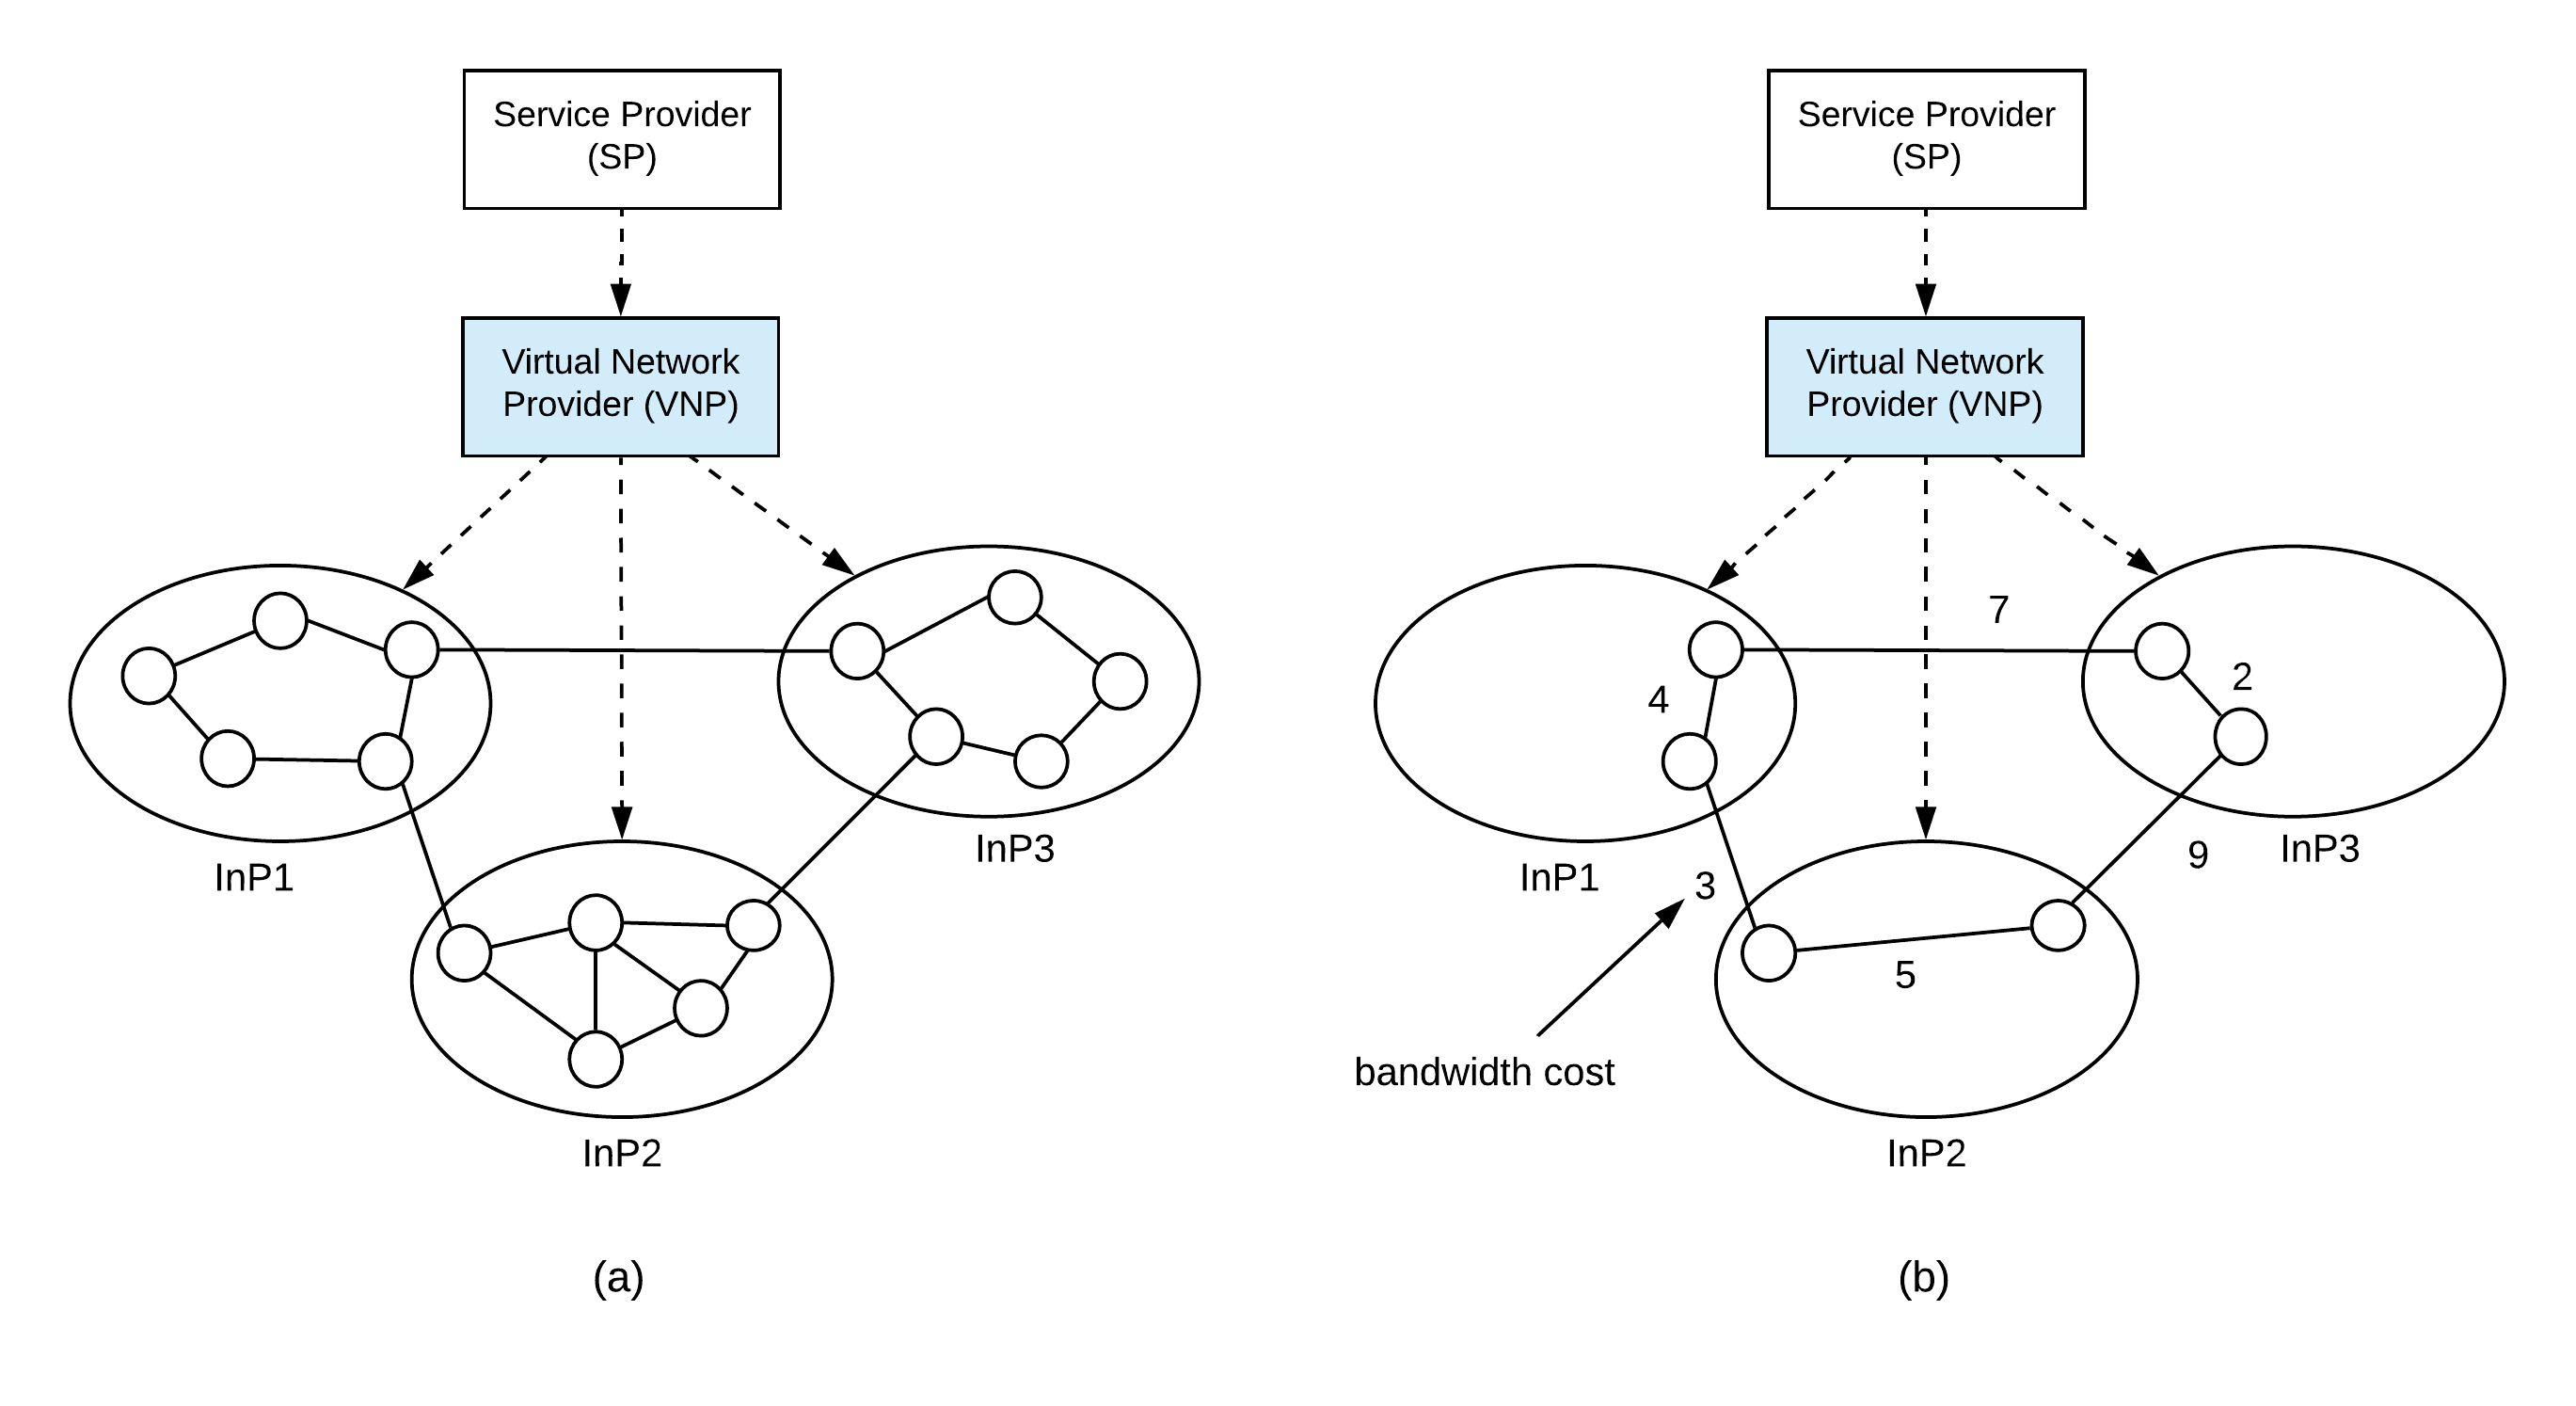
\includegraphics[width=0.9\linewidth]{gfx/multiprov.png}    
  \caption{(a) Virtual network request across multiple InPs using a VN Provider. (b) VNP's view on the substrate network topologies. \citep{dietrich2015multi}}
  \label{fig:multiprov}
\end{figure}

Furthermore, in \citep{dietrich2015multi}, the slice embedding is achieved by subsequently perfoming the following tasks: Firstly, the above-mentioned resource information is sent from the InPs to the VNP, who registers and stores it. Secondly, the VNP matches the service provider request with this collected data. Thirdly, the corresponding partitioning and mapping algorithms are applied (not discussed in this paper). 

In addition, the results prove that this centralized VNE approach provides embedding costs not much higher than in an ideal case scenario (InPs announcing all required information) and a high ratio between the number of slices requested and later allocated. Despite the positive findings, this scenario suffers mainly from scalability, since everything relies on a single centralized authority: the virtual network provider. In addition, it assumes that InPs (if they do so) will be constantly advertising their updated data to the VNP, which can lead to undesired costs.

Therefore, other approaches where the actors benefit from a more scalable and distributed slice embedding need to be further investigated.

\subsubsection{Distributed Slice Embedding}

Many existing solutions \citep{houidi2011virtual}, \citep{dietrich2015multi}, \citep{dietrich2017multi} rely on a centralized party (VNP) that stores the InPs disclosed information and then performs the partition of the virtual network request. However, what if the SPs and InPs are not willing to trust a centralized broker? In that case, this central actor could be removed enabling a direct communication between SPs and InPs, which provides a better system scalability. Distributed network slice embedding has already been investigated in:

\begin{itemize}
	\item In \citep{esposito2013general}, a \textbf{consensus-based auction for distributed slice embedding (CAD)} is proposed. In particular, the physical nodes, which are owned by a single or different InPs, bid on virtual nodes. This value is subsequently stored in a vector $b_i$, where $i$ is the physical node. Afterwards, once the bidding phase concludes, each physical node exchange the bids with its neighbors to reach an agreement for the auctioned virtual nodes. The mentioned bidding can be for a single slice (2 virtual nodes and 1 link) or on the entire slice (multiple virtual nodes and links). In the former, there is a limit on the number of biddable nodes, which although it has a great performance, it provokes multiple iterations (excessive time). Despite in a multi-provider VNE scenario, the latter is more suitable, the InPs willingness to disclose their internal information will hamper the performance. Hence, this approach provides better scalability (decentralization), but it is not proper for our scenario since it does not solve our LID problem.
	\item In \citep{chowdhury2010polyvine}, a \textbf{policy-based inter-domain VN embedding framework (PolyViNE)} is presented. In PolyViNE, each InP embeds part of the VN request under its internal policies, while they cooperate with other InPs in a decentralized manner. In addition, forward decisions are location-based. For example, in Figure \ref{fig:multi} each virtual node (A,B,C,D), has a prefered geolocation. After that, the matched InPs will receive a notification for embedding the specific virtual node (e.g. InP3 with virtual node D). This whole process starts with the SP sending its VN request to multiple trusted InPs who reply back with the related embedding and its prices (bidding). Then, the SP will choose the most economical embedding. However, since there is no central broker, to ensure performance each SP must know $k^{SP} \geq 1$ InPs and each InP $k^{InP} \geq 1$ InPs. Also, most of the time a complete VN is not mappable by a single InP. In this case, the InP embeds its part and forwards the other to a known InP. \newline
Despite, PolyViNE introduces a decentralized approach dealing with LID and uses the interesting location-assisted embedding, it has some drawbacks that need to be covered. Firstly, each InP has an extra overhead in communicating the rest of the request when the VN is not fully mapped. Secondly, the bidding to provide a competitive market is a good idea, but in this scenario, the bids can be publicly known by other InPs. Thus, a better bidding process preventing InPs from revealing its confidential data is needed. Finally, the requirement that SPs and InPs must know at least 1 InPs can lead to an application poor performance.
	
\begin{figure}[bth]
	\centering
	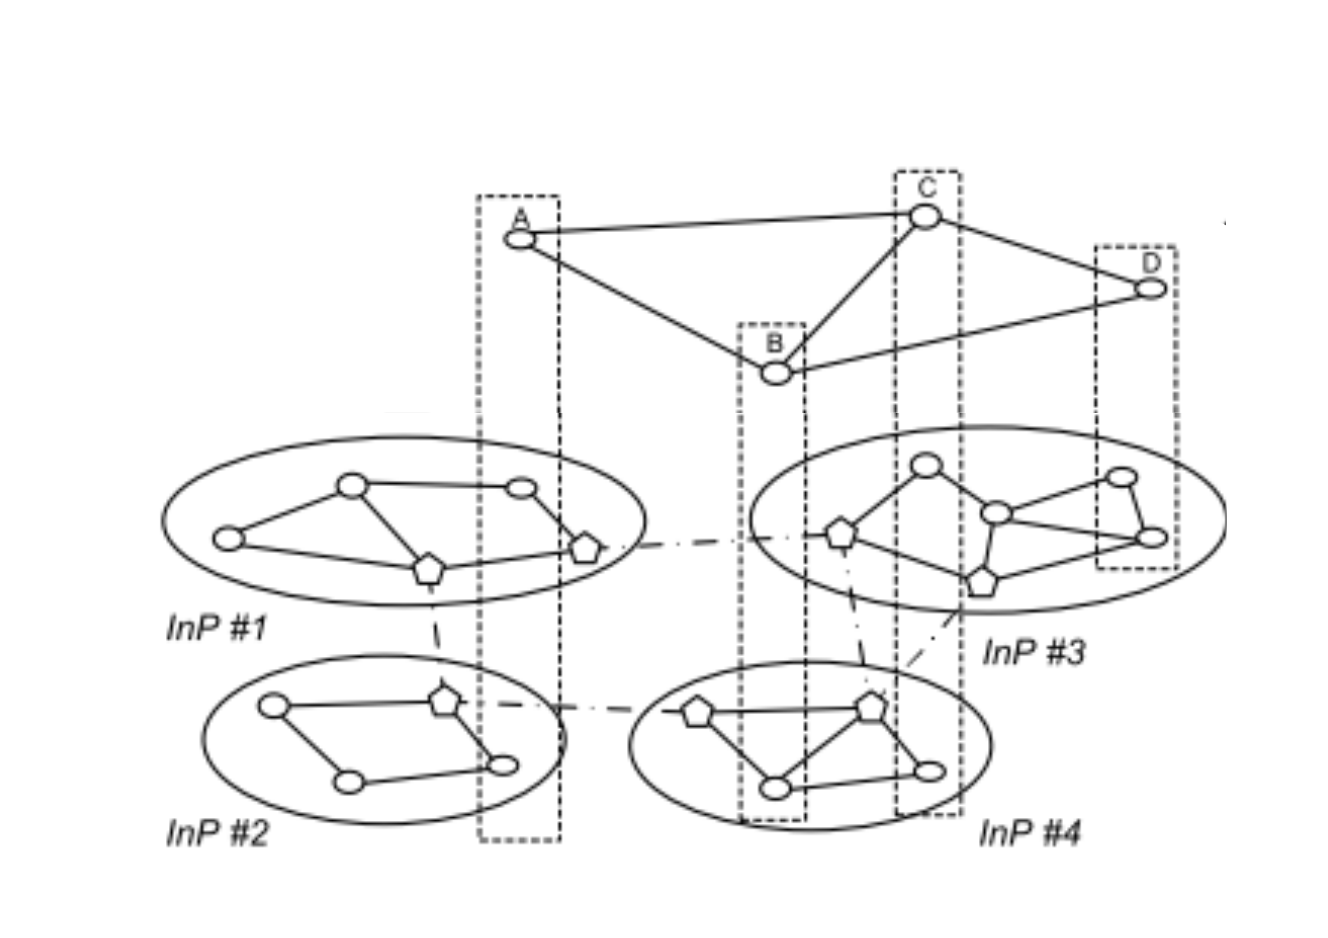
\includegraphics[width=0.6\linewidth]{gfx/multi.png}    
  	\caption{Multi-provider virtual network embedding \citep{chowdhury2010polyvine}}
  	\label{fig:multi}
\end{figure}

\item Finally, in \citep{zaheer2010multi}, an \textbf{automated service negotiation framework (V-Mart)} is implemented. The V-Mart is also decentralized and based on an auction mechanism, the Vickrey auction model.
Though this approach ensures a fair market, thanks to the Vickrey auction model, it does not guarantee performance. The reason is that the VNE process deployed is a second-stage auction where explicitly all the InPs need to interact during the VN embedding. Thus, the VNE results in a high-demanding task. In addition, the sealed-bid is proposed to be done by a trusted 3rd party, which will cause that our application suffers again from centralization issues. Nevertheless, the main V-Mart shortcoming is that it does not solve the LID problem, since it does not enforce inter-domain policies, and the bids and the bidders are at the end known. This disclose once more information that InPs may prefer to keep as confidential.

\end{itemize}
	
All the above related work on decentralized VNE, uses a bidding mechanism to reach an agreement between the SPs and InPs. Therefore, in the next section we will further investigated the fair-price Vickrey auction model, through adapting it to our multi-domain VNE with LID.

\subsubsection{Vickrey Auction Model}

(ASK: SHOULD I MOVE BACKGROUND TO HERE? OR EXPLAIN EVERYTHING IN BACKGROUND?) 
Study \citep{ausubel2006lovely} with equations and everything?
Service negotation has already been examined in \citep{hausheer2005peermart}, \cite{ogston2002peer}, who have worked with diverse auctions platforms. However, as discussed in the background \ref{vickrey}, the Vickrey auction model is the most suitable for our VNE environment.

\section{Analysis of Related Work}

Through relevant examples in supply chain management, as the presented in section \ref{manufacturing}, we can observe the extraordinary potential of blockchain in areas, where entities are willing to exchange data without trusting a third party. Despite the research does not include detailed specifications, such as the blockchain's type or mining strategy, a useful system design has been provided. In addition, some of the main benefits compared to centralized technologies are observed:

\begin{itemize}
	\item \textbf{Disintermediation:} Thanks to the consensus mechanisms, blockchain runs without a central administrator. Thus, intermediaries are not required for realizing transactions which suppresses all the significant costs of involving middle-parties \citep{mainelli2015sharing}. For instance, in the last example, users were able to transfer ownership, by signing the product's contract, without the need of a third party.
	\item \textbf{Autonomy:} After an owner deploys a smart contract on the BC, it is then maintained by all the participating users, and not only by its creator.
	\item \textbf{Data management and redundancy:} Blockchain helps us in coordinating, validating and storing the distributed data in a decentralized manner. It also provides redundancy since users own the same data, e.g. databases backup in centralized systems. 
	\item \textbf{Unconstrained technology:} As actors can define and establish their own rules (smart contracts), new business models open up.
	\item \textbf{Privacy:} Thanks to cryptography, users can interact with untrusted partners. For example, in the above example, all actors can coordinate its services through the PLM process, which before would have been impossible as they do not trust each other.
    \item \textbf{Transparency and integrity:} All the changes that are made to the contract data are directly visible to the other users. In addition, once a transaction is executed, its immutable since it cannot be altered or deleted.
	
\end{itemize}

On the other hand, in the second part of this chapter, we have investigated related work on multi-provider VNE suffering from LID. Table \ref{tab:Comparison} provides a comparison for each of the approaches presented before. 

\begin{table}[bth]
	\myfloatalign \footnotesize
	%18 columns
	\begin{tabularx}{\textwidth}{>{\raggedright\arraybackslash}p{3.5cm} >{\raggedright\arraybackslash}p{1cm}p{0.65cm}p{0.65cm}p{0.65cm}p{0.65cm}p{0.65cm}p{0.65cm}p{0.65cm}p{0.65cm}p{0.65cm}p{0.65cm}p{0.65cm}}
	\textbf{Approach} & \textbf{System} & \rot{\textbf{Scalability}}  & \rot{\textbf{Trusted third party (TTP)}} & \rot{\textbf{Sealed bidding}} & \rot{\textbf{Bid exchange between InPs}} & \rot{\textbf{LID problem solved}} & \rot{\textbf{Location-assisted VNE}} & \rot{\textbf{User notified}} & \rot{\textbf{S-performance}} & \rot{\textbf{L-performance}} & \rot{\textbf{Low VNE cost}} & \rot{\textbf{Low cost (\euro)}}\\ 
		\hline
		Multi-provider VNE framework with VNP \citep{dietrich2015multi} & C & \xmark & \cmark & \xmark & \xmark & \cmark & \cmark & \xmark & \cmark & \xmark & \cmark & \xmark \\ \hline
		CAD - Consensus-based auction for distributed slice embedding \citep{esposito2013general}   &  D & \cmark & \xmark & \xmark & \cmark &  \xmark & \xmark & \xmark & \xmark & \cmark & \xmark & \cmark \\ \hline
		PolyViNE - Policy-based inter-domain VN embedding framework \citep{chowdhury2010polyvine}   &  D & \cmark & \xmark & \xmark & \cmark &  \cmark & \cmark & \cmark & \xmark & \cmark & \cmark & \cmark \\ \hline
		V-mart - Automated service negotiation framework \citep{zaheer2010multi}   &  D & \cmark & * & \cmark & \xmark & \xmark & \xmark & \cmark & \xmark & \xmark & \xmark & \xmark \\
		\hline
	\end{tabularx}
		\caption{Comparison of virtual network embedding approaches - Overview for system features implemented as \textit{yes} (\cmark), \textit{no} (\xmark), \textit{to some extent} (*). Abbreviations: \textit{D} = decentralized, \textit{C} = centralized, \textit{L-performance} = large scenario performance and \textit{S-performance} = small scenario performance.}
	\label{tab:Comparison}
\end{table}

First of all, we can observe that decentralized systems provide obviously a better scalability because the application does not rely on a single point. In centralized systems, this central entity has to be trusted since it stores and manages all the information. Despite being a decentralized system, \cite{zaheer2010multi} uses to some extent a trusted third party (TTP). This is because, it is the only approach that offers sealed-bidding between users, although using a central entity or TTP. We also notice that in \cite{esposito2013general}, \cite{chowdhury2010polyvine} the bids are exchanged between InPs to cooperate in the VN embedding, which results in undesired computational costs. In contrast, centralized systems \citep{dietrich2015multi}, perform the service negotiation without using auctions, since they trust a middle-party managing these operations.

Moreover, one of our main challenges in the multi-provider VNE scenario is to solve the limited information disclosure issues. We notice that \citep{dietrich2015multi}, \citep{chowdhury2010polyvine} deal with the problem, accessing public information not considered confidential and performing the VNE under its internal policies respectively. In addition, they provide location-assisted VNE, which facilitate the VN request partitioning across different InPs. The last, it also introduces a notification system, where the InPs gets notified upon VN request, which avoids time spending in request synchronization. 

In general, centralized systems provide a better throughout in small scenarios since all the information is managed by a central entity. Hence, data sharing or user's cooperation is not needed before performing any operation. Conversely, decentralized systems benefit from large scenarios. Firstly, because the more users participating in an auction, the more competitive the market is. Secondly, all the activities are diversified, and thus, the decision-making is more efficient. 

Finally, we classified costs into virtual network embedding and economic ones. Overall, we observe that VNE costs are lower when using a centralized system \citep{dietrich2015multi}, although when the parties are efficiently coordinated in a decentralized scenario, the costs are also extremely reduced \citep{chowdhury2010polyvine}. Concerning economic costs, they are obviously higher when a centralized system is used, as the application performance depends only on a central entity, which needs to be financed for their computational and maintaining costs.

\section{Summary}

After comparing the different VNE approaches exposed throughout this chapter, we find out that each of them introduces innovate features to deal with network virtualization. However, there is no single solution that satisfies at the same time the following requirements:

\begin{itemize}
	\item Scalability.
	\item LID problem approached with data confidentiality.
	\item L-performance.
	\item Computational and economic low costs.
\end{itemize}

Therefore, after spotting the main benefits of integrating blockchain in real-scenarios, we predict that blockchain could fulfill the above-mentioned VNE demands, by giving rise to a new decentralized, automated and secure system between the SPs and InPs.

%*****************************************
\chapter{Design}
\label{ch:design}
%*****************************************

\hint{This chapter should describe the design of the own approach on a conceptional level without mentioning the implementation details. The section should have a length of about five pages.}

1. Types of blockchain (permissionless and permissioned) economical reasons: cost, maintenance, computing power...
2. Scenario, architecture
3. Notification system (P/S)
4. Mining
5. Authentication system
6. Vickrey auction model

1. Invite People to the private BC. Users fixed amount of Ether ( Proof of Stake). Garzik, J. 2015. "Public Versus Private Blockchains.
1. Since it is a disruptive technology, apparently it seems that blockchain could improve many existing systems. However, is it suddenly blockchain the only way of approaching scalability, security or data handling between organizations? Or why is a blockchain better than a traditional database? The truth of it is that there is not a single solution or better technology than the others, it just depends on user's requirements. Thus, it is important to understand when blockchain could replace existing infrastructures. For this purpose, in \ref{fig:bcFlowchart} we present a flowchart, which pretends to guide users in determining whether blockchain is the appropriate solution to resolve their problems.

EXPLAIN FIGURE! ALSO TABLE COMPARING TYPES OF BC.
Nevertheless, the technology still faces lots of challenges, such as scalability or incorporating external information, which will be later further investigated.
\begin{figure}[bth]
	\centering
	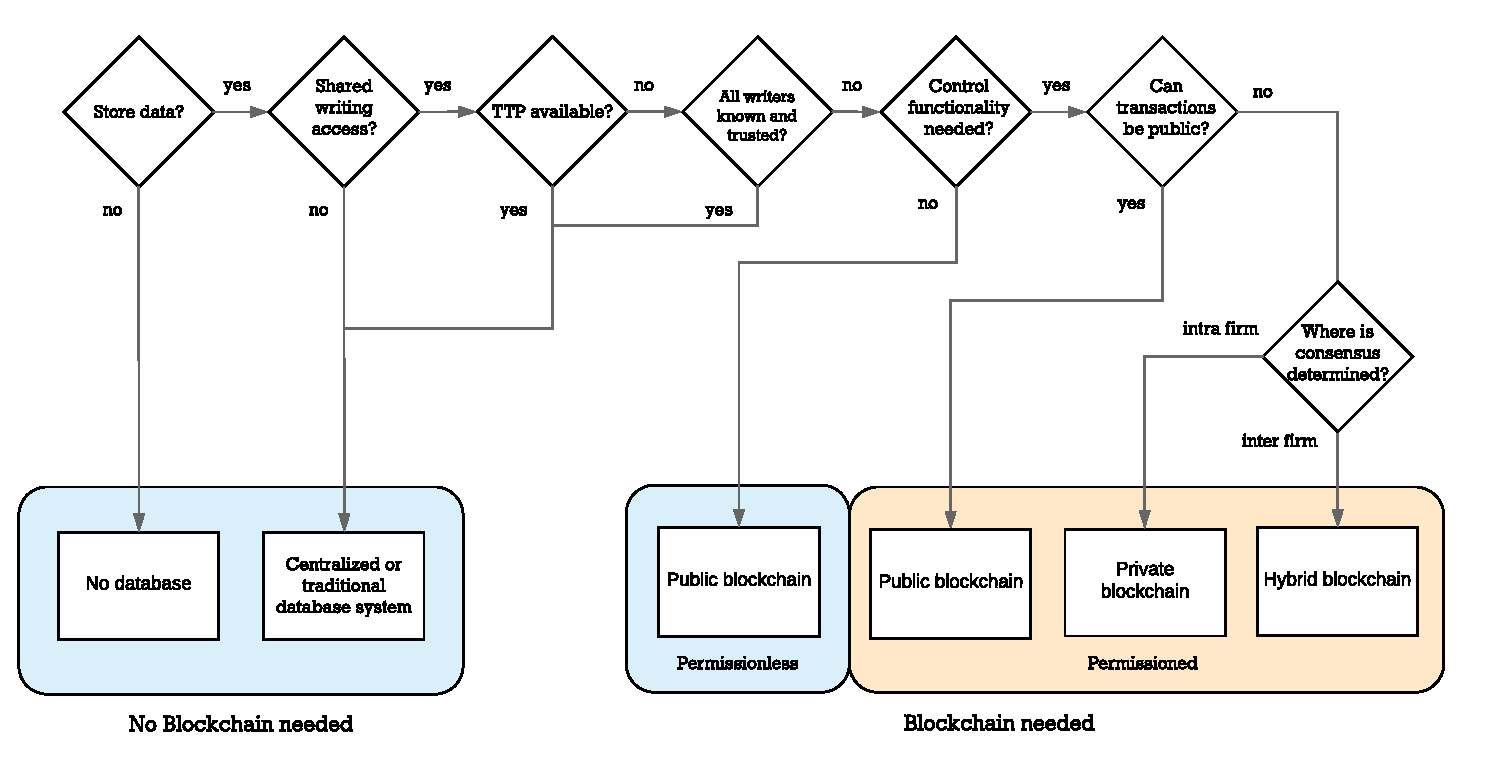
\includegraphics[width=1\linewidth]{gfx/bcFlowchart}    
  	\caption{Flow-chart to determine whether blockchain is the suitable solution \citep{wust2017you}}
  	\label{fig:bcFlowchart}
\end{figure}

1. PROBLEMS: -  The participants of a SCM vary greatly across different supply
chains and the same peers might take different roles across different supply chains. - This reasoning leaves us with the question whether all writers
can be trusted. 

2.A DApp has its backend code running on a decentralized peer-to-peer network. Contrast this with an app where the backend code is running on centralized servers. A DApp can have frontend code and user interfaces written in any language (just like an app) that can make calls to its backend. Furthermore, its frontend can be hosted on decentralized storage such as Swarm or IPFS.

What can be externally extracted from a contract? Since value transfers cannot be blinded in Ethereum, anyone can see the value and therefore the highestBid. Sol: We can just see the address. That's a problem if there are just a few users. Do research on amount of users needed to solve the problem.

4. Mining from users or supernode? Start with supernodes (like in Bitcoin at the beginning), when more users maybe a user say he want to become a miner (gets the privileges and anonimity increased)

6. In this case, our auction procedure will start with the SP requesting a virtual network (a graph of virtual nodes) along with an upper bound, the last being the maximum amount of money the SP is willing to pay. Then, the InPs will estimate the request requirements (e.g: nodes availability or costs) in their infrastructure and thereafter submit their bids. In other words, the InPs will be sellers submitting bids and SPs the consumers requesting a service.

It is important to note that in our scenario, similar to \citep{zaheer2010multi}, the \textbf{lowest auction} will win and not the highest. The reason is that at the end the SPs is who will pay the bid value. For instance, suppose that all the InPs make an offer close to the upper bound specified by the SP. If the highest bid wins, the SPs will always end-up paying approximately its upper bound (unfair). However, if the lowest bid wins, the system ensures that the InPs submits a bid proportional to the real cost since it will be the minimum amount of money that they could earn.
Explain that an auction could use a multi-dimensional process (more parameters).

6. Package pricing or volume discount?

Thanks to the blockchain, more precisely to Ethereum and smart contracts, the untrustworthy VNP could be replaced with a secure, flexible and coordinated end-system. Hence, InPs disclosed information will be kept confidential (public/private key cryptography) in the blockchain and just accessible for its desired users. which could be accomplished through a limited time auction.

During this paper, the Ethereum blockchain will be used to perform a service negotiation (Vickrey auction) and later to track its possession throughout the supply chain process. This will be exemplified by a web application implementation, focused on network slicing. Thus, blockchain strengths and weaknesses will be further investigated.

The blockchain technology, in particular, secure smart contracts on the Ethereum platform, will be used to approach a real-world scenario. A decentralized application (third category) that enhances supply chain performance, will be implemented. More precisely, network virtualization providers and customers will improve its communication, through the use of a web application (front-end) connected to the blockchain (back-end).

We do not claim that our approach is the best or the only way
of performing VN embedding. On the contrary, it is more an add-on feature that can be merged with most of the existing solutions. In this scenario, the main goals are to remove the middleware or virtual network provider, by using a new prominent technology such as blockchain. Thus, a new decentralized, automated and secure system between the SPs and InPs will be created, which benefits from the blockchain potentials. Furthermore, to the best of our knowledge, this is the first approach using blockchain in the network virtualization context, and thanks to smart contract's flexibility, it can serve as a starting point for upcoming investigations.

\section{Requirements and Assumptions}

e.g: Flexibility, fair price negotiation, trustworthy, transparent ... And explain each point
Assumption that intra-domain virtual links cost is almost 0. Having the virtual link cost from EC2 Amazon and the BW we could determine it...

\section{System Overview}

\subsection{Component 1}

\subsection{Component 2}

\section{Summary}

%*****************************************
\chapter{Implementation}

1. How a contract is compiled in to the Ethereum BC.
2. Technologies used (GETH vs ETH NW, web3, Solidity, truffle).
(The Genesis block is the first block in a blockchain. It is always hardcoded in the blockchain).
3. Authentication 
4. Component relations in the source code
5. Code examples

3.Investigate web3.eth.sign(web3.eth.accounts[0], address), the address should be unlocked. How this is possible?

\label{ch:implementation}
%*****************************************

\hint{This chapter should describe the details of the implementation addressing the following questions: \\ \\
1. What are the design decisions made? \\
2. What is the environment the approach is developed in? \\
3. How are components mapped to classes of the source code? \\
4. How do the components interact with each other?  \\
5. What are limitations of the implementation? \\ \\
The section should have a length of about five pages.}


\section{Design Decisions}


\section{Architecture}

\section{Interaction of Components}

\section{Summary}

%*****************************************
\chapter{Evaluation}
\label{ch:evaluation}
%*****************************************
\hint{This chapter should describe how the evaluation of the implemented mechanism was done. \\ \\
1. Which evaluation method is used and why? Simulations, prototype? \\
2. What is the goal of the evaluation? Comparison? Proof of concept? \\
3. Wich metrics are used for characterizing the performance, costs, fairness, and efficiency of the system?\\
4. What are the parameter settings used in the evaluation and why? If possible always justify why a certain threshold has been chose for a particular parameter.  \\
5. What is the outcome of the evaluation? \\ \\
The section should have a length of about five to ten pages.}

Test scenario with Real users using our application.

\section{Goal and Methodology}

\section{Evaluation Setup}

\section{Evaluation Results}

\section{Analysis of Results}


%*****************************************
\chapter{Conclusions}
\label{ch:closure}
%*****************************************

\hint{This chapter should summarize the thesis and describe the main contributions of the thesis. Subsequently, it should describe possible future work in the context of the thesis. What are limitations of the developed solutions? Which things can be improved?
The section should have a length of about three pages.}

\section{Summary}

\section{Contributions}

\section{Future Work}

IOTA-TANGLE
BigchainDB
The Front-end application could be hosted in a decentralized storage such as IPFS or SWARM.
BC storing chunks of data

\section{Final Remarks}
